\documentclass[12pt.a4paper]{article}
\usepackage[utf8]{inputenc}
\usepackage[spanish]{babel}
\usepackage{amsmath}
\usepackage{graphicx} 
\usepackage{geometry}
\usepackage{float} % Para controlar la ubicación de las figuras
\usepackage{tabularx}
\usepackage{titlesec}
\usepackage{lipsum}
\usepackage{geometry} % Paquete para controlar los márgenes
\usepackage[colorlinks= true, allcolors=blue]{hyperref}
\usepackage{fancyhdr}
\usepackage{tikz}
\usepackage{lastpage}

% Configuración de márgenes
\geometry{
    left=2.5cm,  % Margen izquierdo
    right=2.5cm, % Margen derecho
    top=3cm,     % Margen superior
    bottom=3cm   % Margen inferior
}

\pagestyle{fancy}
\fancyhf{}
\renewcommand{\headrulewidth}{0pt}

\fancyhead[R]{
    \begin{tikzpicture}[remember picture,overlay]
        \node[anchor=north east,xshift=-5mm,yshift=-5mm] at (current page.north east) {
            \fbox{
                \begin{tabular}{r l}
                    Revisión: & 01 \\
                    Clave: & DOC-001 \\
                    Página: & \thepage\ de \pageref{LastPage}
                \end{tabular}
            }
        };
    \end{tikzpicture}
}

\titleformat{\section}{\normalfont\Large\bfseries}{\thesection}{1em}{}
\titleformat{\subsection}{\normalfont\large\bfseries}{\thesubsection}{1em}{}
\titleformat{\subsubsection}{\normalfont\normalsize\bfseries}{\thesubsubsection}{1em}{}

\begin{document}

% Portada
\begin{titlepage}
\centering
{\bfseries\LARGE Universidad de Málaga\par}
\vspace{1cm}
{\scshape\Large ETSI Informática\par}
\vspace{2cm}
{\scshape\Huge Documento General de Requisitos Mini PIM}
\vspace{2cm}
\begin{figure}[H]
    \centering
     
\includegraphics[width=0.25\linewidth]{umaLogo.png}
\end{figure}
\vfill
{\Large Diego Sicre Cortizo\par}
{\Large Pablo Ortega Serapio\par}
{\Large Angel Nicolás Escaño López\par}
{\Large Francisco Javier Jordá Garay\par}
{\Large Janine Bernadeth Olegario Laguit\par}
\vspace{1cm}
{\Large Grupo 01}
\vfill
{\Large Octubre 2024}

\end{titlepage}

\thispagestyle{empty} %quita el numero de la primera pagina
\tableofcontents
\thispagestyle{empty} %quita el numero de la primera pagina


\newpage
\setcounter{page}{1}
\section{Introducción}

\subsection{Objetivos}

El objetivo de este \textit{Documento General de Requisitos} es recoger, analizar y definir las características y necesidades de alto nivel del sistema Mini PIM (Product Information Management). Este documento se centra en describir las expectativas de cada una de las partes interesadas en el proyecto, así como de los usuarios finales, y justifica por qué estas necesidades existen. Además, se exploran las funcionalidades necesarias para el desarrollo del sistema y se establecen especificaciones claras para su implementación. Los detalles de cómo el sistema Mini PIM cumplirá con estas necesidades se ampliarán en los casos de uso y en las especificaciones adicionales.

\subsection{Alcance}

Este \textit{Documento General de Requisitos} proporciona una descripción breve del ámbito que cubre el sistema Mini PIM, destacando su relación con otros proyectos de gestión de información de productos para PyMEs y su conexión con plataformas de integración externas como Amazon. El documento establece los criterios de escalabilidad y requisitos funcionales esenciales, sentando las bases para la estructura de crecimiento del sistema, permitiendo futuras actualizaciones y estableciendo el marco en el que el sistema debe desarrollarse.


\subsection{Definiciones, acrónimos y abreviaturas}

\begin{itemize}
    \item \textbf{PIM}: Product Information Management (Gestión de Información de Producto)
    \item \textbf{SKU}: Stock Keeping Unit - Identificador único de producto
    \item \textbf{GTIN}: Global Trade Item Number - Identificador global para productos en comercio electrónico
    \item \textbf{Assets}: Recursos digitales asociados a productos, como imágenes, videos y documentos PDF
    \item \textbf{API}: Application Programming Interface - Interfaz para la integración con sistemas externos
\end{itemize}

\subsection{Referencias}

\begin{itemize}
    \item Estándar de accesibilidad WCAG 2.2 (nivel AA) para asegurar la accesibilidad del sistema.
    \item Especificaciones técnicas para la integración con Amazon Prime y otros canales de venta: Buy with Prime.
    \item Documentación interna de Plytix sobre la estructura y requisitos del sistema Mini PIM.
\end{itemize}

\subsection{Resumen}

Este \textit{Documento General de Requisitos} organiza y estructura los contenidos para guiar la implementación del sistema Mini PIM de manera eficiente. Cada sección del documento se centra en un aspecto específico del sistema, comenzando con las directivas del proyecto, una breve descripción de los participantes y los usuarios, una visión general del producto y una identificación de requisitos funcionales y no funcionales, hasta llegar al modelo de dominio que lo describe. Esta organización facilita la implementación, gestión y evolución de este.

\section{Directivas del proyecto}

\subsection{Oportunidad de negocio}

En el mercado actual, las pequeñas y medianas empresas (PyMEs) enfrentan una desventaja competitiva frente a las grandes empresas en cuanto a la gestión y exposición de sus productos en plataformas de comercio electrónico. Las soluciones profesionales de gestión de información de productos (PIM) existentes en el mercado son, en su mayoría, costosas y complejas, lo que las hace inaccesibles para muchas PyMEs. La oportunidad de negocio radica en desarrollar un sistema PIM asequible, eficiente y fácil de usar que permita a estas empresas gestionar de manera centralizada la información de sus productos, assets y relaciones, y exportar datos a distintos canales de venta, aumentando así su competitividad en el mercado digital.

\subsection{Descripción del problema}

La falta de herramientas accesibles para gestionar información de productos impide que las PyMEs compitan en igualdad de condiciones contra las grandes corporaciones, reduciendo su visibilidad y eficiencia, lo que podría resolverse con una plataforma que centralice y optimice estas gestiones e integraciones con canales de venta externos.

\subsection{Descripción del producto}

Mini PIM es un sistema de gestión de información de productos diseñado específicamente para pequeñas y medianas empresas (PyMEs) que buscan una solución accesible y asequible para centralizar la administración de sus productos y assets digitales. El producto permite a las PyMEs gestionar eficientemente sus catálogos de productos, relaciones y recursos digitales, además de integrarse automáticamente con plataformas de venta externas como Amazon para aumentar la visibilidad y el alcance en el mercado digital.

El Mini PIM se diferencia de sus competidores por ofrecer planes de suscripción flexibles y escalables, adaptados a las necesidades y capacidades de las PyMEs, garantizando una gestión eficiente y optimizada sin los altos costos ni la complejidad técnica que suelen tener las soluciones PIM dirigidas a grandes corporaciones.


\section{Descripción de Participantes y Usuarios}

\subsection{Resumen de los Participantes}

\begin{itemize}

    \item \textbf{Canales de venta (Amazon, AliExpress, ...)} \\
        Encargados de realizar la venta de los objetos que, mediante el uso del sistema, serán publicados y puestos a la venta.
    \item \textbf{Canales de pago (PayPal y Stripe)} \\
        Asegurarán que las suscripciones de pago de los usuarios sean cobradas correctamente y que se puedan modificar las suscripciones abiertamente.
    \item \textbf{Jefe o gerente de la empresa} \\
        Es el owner, quien será el encargado de proveer una cuenta a cada uno de los trabajadores de la tienda.
    \item \textbf{Soporte Técnico} \\
        Es capaz tanto de simular una cuenta de \textit{Owner} como de \textit{User} con fines de soporte técnico.
    \item \textbf{Empleado} \\
        Es la cuenta que utilizará un trabajador normal, con la capacidad de gestionar los productos de una tienda.
    \item \textbf{Plytix Admin} \\
        Es el encargado de crear las cuentas \textit{Owner} para una empresa y las cuentas \textit{Agente} para soporte técnico.
\end{itemize}

\subsection{Resumen y Entorno de los Usuarios}

\begin{tabularx}{\textwidth}{|l|X|l|}
    \hline
    \textbf{Nombre} & \textbf{Descripción} & \textbf{Participante} \\
    \hline
    Owner & Es el jefe de la tienda, encargado de proveer una cuenta a cada trabajador & Se asocia al participante Jefe o Gerente \\
    \hline
    Agente & Puede simular tanto una cuenta de \textit{Owner} como de \textit{User} & Se asocia al participante Soporte Técnico \\
    \hline
    User & Representa a un trabajador que gestiona productos de la tienda & Se asocia al participante Empleado \\
    \hline
\end{tabularx}

\subsection{Perfiles de los Participantes}

\subsubsection{Jefe / Gerente}

\begin{itemize}
    \item \textbf{Representante:} Jefe o gerente de la empresa.
    \item \textbf{Descripción:} Es el jefe o gerente de una empresa.
    \item \textbf{Tipo:} Alto cargo ejecutivo.
    \item \textbf{Responsabilidades:}
    \begin{itemize}
        \item Gestionar el funcionamiento de la empresa.
        \item Encargado de crear las cuentas \textit{User} para los trabajadores.
    \end{itemize}
    \item \textbf{Criterio de Éxito:} Crear y gestionar correctamente las cuentas \textit{User}, mantener buena comunicación con soporte técnico para gestionar eficientemente los productos de la empresa.
    \item \textbf{Comentarios:} Encargados de crear las cuentas tipo \textit{User} y realizar las gestiones de pago.
\end{itemize}

\subsubsection{Trabajador}

\begin{itemize}
    \item \textbf{Representante:} Trabajador.
    \item \textbf{Descripción:} Es un trabajador de una empresa.
    \item \textbf{Tipo:} Equipo laboral de una empresa.
    \item \textbf{Responsabilidades:}
    \begin{itemize}
        \item Utilizar y gestionar sus cuentas \textit{User}.
        \item Gestionar los productos de la tienda.
    \end{itemize}
    \item \textbf{Criterio de Éxito:} Gestionar correctamente tanto la organización de los productos como su envío a los canales de venta.
    \item \textbf{Comentarios:} Los trabajadores sólo pueden controlar cuentas \textit{User}, sin privilegios de creación ni modificación de cuentas.
\end{itemize}

\subsubsection{Soporte Técnico}

\begin{itemize}
    \item \textbf{Representante:} Soporte técnico de Plytix.
    \item \textbf{Descripción:} Encargado de soporte técnico.
    \item \textbf{Tipo:} Equipo de soporte técnico.
    \item \textbf{Responsabilidades:}
    \begin{itemize}
        \item Gestionar el funcionamiento de una cuenta Plytix.
        \item Corregir errores en el sistema y ayudar a las empresas.
    \end{itemize}
    \item \textbf{Criterio de Éxito:} Resolver problemas y mantener un correcto funcionamiento del software.
    \item \textbf{Comentarios:} Representantes de soporte técnico pueden utilizar cualquier tipo de cuenta para solucionar problemas.
\end{itemize}

\subsubsection{Plytix Admin}

\begin{itemize}
    \item \textbf{Representante:} Administrador de Plytix
    \item \textbf{Tipo:} Representante de Plytix / Alto cargo ejecutivo
    \item \textbf{Responsabilidades:}
    \begin{itemize}
        \item Crear las cuentas \textit{Owner} de las empresas.
        \item Gestionar y crear cuentas \textit{Agente} para soporte técnico.
    \end{itemize}
    \item \textbf{Criterio de Éxito:} Gestionar correctamente cuentas \textit{Owner} y \textit{Agente}.
    \item \textbf{Entregables:} Cuentas \textit{Owner} y soporte técnico para las empresas.
    \item \textbf{Comentarios:} El administrador tiene todos los permisos.
\end{itemize}

\subsection{Perfiles de Usuario}

\subsubsection{Owner}

\begin{itemize}
    \item \textbf{Representante:} Owner.
    \item \textbf{Descripción:} Es el jefe o gerente de una empresa.
    \item \textbf{Tipo:} Alto cargo ejecutivo.
    \item \textbf{Responsabilidades:}
    \begin{itemize}
        \item Crear cuentas para los trabajadores.
        \item Gestionar el plan de suscripción de la empresa.
    \end{itemize}
    \item \textbf{Criterio de Éxito:} Mantener un número adecuado de trabajadores y maximizar ventas.
    \item \textbf{Comentarios:} El \textit{Owner} es la cuenta principal de la empresa.
\end{itemize}

\subsubsection{Agente}

\begin{itemize}
    \item \textbf{Representante:} Agente.
    \item \textbf{Descripción:} Personal de servicio técnico de Plytix.
    \item \textbf{Tipo:} Servicio técnico.
    \item \textbf{Responsabilidades:}
    \begin{itemize}
        \item Gestionar la funcionalidad de cuentas empresariales.
        \item Solucionar problemas en cuentas Plytix.
    \end{itemize}
    \item \textbf{Criterio de Éxito:} Solventar adecuadamente los errores que surjan a los clientes durante el uso del sistema.
    \item \textbf{Comentarios:} Agentes pueden adoptar permisos de \textit{Owner} y \textit{User} para solucionar problemas.
\end{itemize}

\subsubsection{User}

\begin{itemize}
    \item \textbf{Representante:} Usuario.
    \item \textbf{Descripción:} Representa a los trabajadores de la empresa.
    \item \textbf{Tipo:} Equipo de trabajo.
    \item \textbf{Responsabilidades:}
    \begin{itemize}
        \item Gestionar productos de la tienda.
        \item Mover productos a los canales de venta mediante CSV o APIs.
        \item Editar datos de productos.
    \end{itemize}
    \item \textbf{Criterio de Éxito:} Mantener actualizada la información y gestionar los productos, sus atributos y relaciones de forma adecuada.
    \item \textbf{Comentarios:} Los usuarios sólo gestionan productos, sin acceso a gestión de cuentas o suscripciones.
\end{itemize}

\subsection{Alternativas y Competencia}

\begin{itemize}
    \item Plataformas E-Commerce.
    \item Cualquier plataforma PIM.
    \item Otro software de gestión de inventario.
\end{itemize}


\section{Visión General del Producto}

\subsection{Entorno de Despliegue}

\subsubsection{Entorno para la Implementación del Sistema Actual}
El sistema se desplegará en un entorno SaaS adecuado para PyMEs, donde los usuarios podrán gestionar la información de sus productos y sincronizarlos con los distintos canales de venta. Se garantizará que el sistema cumpla con los requisitos de seguridad, escalabilidad y disponibilidad, necesarios para operar en plataformas de venta en línea.

\subsubsection{Aplicaciones Colaboradoras}
El Mini PIM de Plytix se integrará con diversas aplicaciones de comercio electrónico, tales como Amazon y Shopify, con el objetivo de facilitar la exportación de datos de productos hacia estos canales de venta. También podrá conectarse a plataformas internas de gestión de inventarios o de catálogo, que los clientes utilicen para preparar sus datos de productos antes de la sincronización, de las cuales podrán importar información en formato CSV.

\subsection{Resumen de Características}

\begin{table}[H]
\centering
\begin{tabular}{|l|p{10cm}|}
    \hline
    \textbf{Sistema} & Mini PIM \\
    \hline
    \textbf{Beneficios para el Cliente} & Permite a las PyMEs gestionar y centralizar la información de sus productos en un solo lugar, optimizando la organización y facilitando la exportación de estos datos a los canales de venta en línea. Aumenta la eficiencia operativa en la actualización y publicación de productos. \\
    \hline
    \textbf{Características de Soporte} & 
    \begin{itemize}
        \item CRUD (Crear, Leer, Actualizar y Eliminar) de productos y características.
        \item Exportación directa de productos a plataformas de comercio electrónico.
        \item Automatización para sincronizar y actualizar la información de productos en varios canales.
    \end{itemize} \\
    \hline
\end{tabular}
\end{table}


\subsection{Suposiciones y Dependencias}

\subsubsection{Factores Externos que Tienen un Efecto en el Producto, pero No son Restricciones Obligatorias}
Factores como los cambios en las políticas de integración de los canales de venta (por ejemplo, Amazon o Shopify) y las actualizaciones en las regulaciones de privacidad de datos pueden afectar las funcionalidades de exportación del sistema, aunque no se consideran restricciones obligatorias en su diseño inicial.

\subsubsection{Suposiciones que Asume el Equipo en Torno al Proyecto}
Se asume que:
\begin{itemize}
    \item Los clientes cuentan con la infraestructura mínima necesaria para acceder al sistema.
    \item Los datos de productos están organizados y en formatos compatibles para su importación al sistema.
    \item La plataforma se mantendrá como una herramienta de soporte para la gestión de productos de PyMEs en mercados internacionales, por lo que se utilizará el ingés americano.
\end{itemize}

\subsection{Precio y Coste}
El sistema funcionará bajo un modelo de suscripción mensual, el cual varía según la cantidad de usuarios que requieran acceso al sistema y el nivel de funcionalidades de soporte para exportación de productos. Los costos de mantenimiento y las actualizaciones periódicas se incluirán dentro del precio de suscripción.

\subsection{Licencias e Instalación}
Mini PIM ofrecerá licencias de suscripción para el uso del sistema, que estarán sujetas a los términos de uso y privacidad de la empresa.
\section{Requisitos Funcionales}
\subsection*{RF1 Gestión de Cuenta}

\begin{itemize}
    \item \textbf{RF1.1 Creación de cuentas Owner} \\
    El sistema debe permitir a los Plytix Admin crear cuentas Owner.
    
    \item \textbf{RF1.3 Creación de cuentas User} \\
    El sistema debe permitir al Owner crear cuentas de usuario para empleados de la empresa (User).

    \item \textbf{RF1.4 Visualizar datos de la cuenta} \\
    El usuario debe poder ver los datos de su cuenta: nombre, logotipo, correo, contraseña, fecha y hora de creación.

    \item \textbf{RF1.5 Actualizar datos de la cuenta} \\
    El usuario debe poder modificar los datos de la cuenta, a excepción de la fecha y hora de creación.

    \item \textbf{RF1.6 Borrar cuenta} \\
    El sistema debe permitir la eliminación de una cuenta a un Owner, siguiendo políticas de seguridad y permisos.

    \item \textbf{RF1.7 Iniciar sesión} \\
    Los usuarios deben poder autenticarse en el sistema introduciendo credenciales válidas.

    \item \textbf{RF1.8 Cerrar sesión} \\
    El sistema debe permitir al usuario cerrar sesión de manera segura.

    \item \textbf{RF1.9 Crear informe de cuenta} \\
    El sistema debe poder generar un informe detallado con la información de la cuenta.
    \begin{itemize}
        \item \textbf{RF1.9.1 Exportar informe de cuenta} \\
        El informe generado debe poder ser exportado en formato .json, incluyendo la información  de: nombre de la cuenta, fecha de creación, número de productos, assets y tamaño utilizado de almacenamiento en bytes, número de categorías de productos y assets, número de atributos de usuario creados, número de relaciones creadas, una lista de los usuarios con su nombre, si existe, y su dirección de correo electrónico.
    \end{itemize}


    \item \textbf{RF1.10 Emulación de cuenta} \\
    El Agente puede emular una cuenta de  \textit{Owner} o  \textit{User} para brindar soporte y verificar problemas específicos de la cuenta.

    \item \textbf{RF1.11 Creación de cuenta Agente} \\
    La cuenta de Agente debe crearse y eliminarse desde el sistema de administración central de Plytix.


    \item \textbf{RF1.12 Capacidad y duración de la cuenta Agente} \\
    El Agente tiene permisos para ver y analizar los datos de productos y assets, pero no puede modificar ni eliminar información de la cuenta a la que brinda soporte y tiene tiempo de vida limitado hasta que se soluciona el problema.
\end{itemize}

\subsection*{RF2 Gestión de Producto}

\begin{itemize}
    \item \textbf{RF2.1 Crear producto} \\
    Todos los usuarios deben poder añadir nuevos productos al sistema, especificando los atributos del sistema: GTIN, SKU, clave, thumbnail y label; los atributos de usuario, hasta 5 opcionales; y las categorías, assets y relaciones.

    \item \textbf{RF2.2 Visualizar producto} \\
    Los productos deben poder ser visualizados con todos sus detalles.

    \item \textbf{RF2.3 Editar producto} \\
    El sistema debe permitir a los usuarios editar la información de los productos existentes.

    \item \textbf{RF2.4 Borrar producto} \\
    Los productos deben poder ser eliminados por los usuarios, siempre y cuando no estén asociados a otras entidades clave del sistema.

    \item \textbf{RF2.5 Importación de productos en plataformas externas} \\
    Los usuarios deben poder importar productos de plataformas externas al sistema.
\end{itemize}

\subsection*{RF3 Gestión de Assets}

\begin{itemize}
    \item \textbf{RF3.1 Crear asset} \\
    Todos los usuarios deben poder subir assets al sistema de tipo: pdf, imágen, vídeo, binario y ejecutable.

    \item \textbf{RF3.2 Visualizar asset} \\
    El sistema debe permitir visualizar los assets almacenados, incluyendo el nombre, su fecha de adición, la asociación con otros productos, su thumbnail, el tipo de archivo y su tamaño.

    \item \textbf{RF3.3 Editar asset} \\
    Los usuarios deben poder modificar las propiedades de un asset.

    \item \textbf{RF3.4 Borrar asset} \\
    Los assets pueden ser eliminados, salvo que estén asociados a un producto.
    \begin{itemize}
        \item \textbf{RF3.4.1 Restricción de borrado de asset} \\
        El sistema debe impedir la eliminación de un asset si está asociado a algún producto.
    \end{itemize}

    \item \textbf{RF3.5 Crear asociación de asset} \\
    Los usuarios deben poder asociar assets a productos en el sistema.

    \item \textbf{RF3.6 Ver asociación de asset} \\
    Las asociaciones de assets con productos deben ser visibles y consultables por los usuarios.

    \item \textbf{RF3.7 Editar asociación de asset} \\
    El sistema debe permitir modificar las asociaciones entre assets y productos.

    \item \textbf{RF3.8 Borrar asociación de asset} \\
    Los usuarios deben poder eliminar asociaciones de assets, siempre y cuando no violen restricciones del sistema.
\end{itemize}

\subsection*{RF4 Gestión de Categorías}

\begin{itemize}
    \item \textbf{RF4.1 Crear categoría} \\
    Todos los usuarios pueden definir categorías.

    \item \textbf{RF4.2 Visualizar categorías} \\
    Las etiquetas creadas deben poder ser visualizadas junto a sus datos: nombre y número de productos asociados.

    \item \textbf{RF4.3 Editar categoría} \\
    El sistema debe permitir la modificación de los datos de las cateogorías existentes.

    \item \textbf{RF4.4 Borrar categoría} \\
    Los usuarios deben poder eliminar cateogorías, a excepción de que estas estén asociadas a otros elementos críticos en el sistema.
\end{itemize}

\subsection*{RF5 Gestión de Relaciones}

\begin{itemize}
    \item \textbf{RF5.1 Crear relación} \\
    Todos los usuarios deben poder crear relaciones entre productos.

    \item \textbf{RF5.2 Ver relación} \\
    Las relaciones entre productos deben ser visibles y accesibles para los usuarios junto a su nombre.

    \item \textbf{RF5.3 Actualizar relación} \\
    El sistema debe permitir la modificación de las relaciones existentes entre productos.

    \item \textbf{RF5.4 Borrar relación} \\
    Los usuarios deben poder eliminar relaciones, siempre y cuando no afecten la integridad de otras funciones del sistema.

    \item \textbf{RF5.5 Relacionar productos} \\
    El sistema debe permitir vincular productos mediante relaciones.
    
    \item \textbf{RF5.6 Modificar datos} \\
    El sistema debe permitir modificar los datos de la relación.
    
\end{itemize}

\subsection*{RF6 Gestión de Atributos}

\begin{itemize}
    \item \textbf{RF6.1 Crear atributo} \\
    Todos los usuarios pueden definir atributos personalizados para los productos con un límite de hasta 5 atributos creados por usuario.

    \item \textbf{RF6.2 Ver atributo} \\
    Los atributos de productos deben ser visibles para los usuarios y mostrarse en los detalles del producto.

    \item \textbf{RF6.3 Editar atributo} \\
    El sistema debe permitir la modificación de los atributos de los productos.

    \item \textbf{RF6.4 Borrar atributo} \\
    Los usuarios deben poder eliminar atributos, siempre y cuando no afecten otras funcionalidades del sistema.

    \item \textbf{RF6.5 Atributos del sistema} \\
    Los atributos del sistema están disponibles para todos los productos de manera predeterminada.
    \begin{itemize}
        \item \textbf{RF6.5.1 Label} \\
        El sistema debe permitir asignar un label a cada producto.

        \item \textbf{RF6.5.2 SKU} \\
        Cada producto debe tener un código único (SKU) que lo identifique.

        \item \textbf{RF6.5.3 GTIN} \\
        El sistema debe gestionar los atributos de GTIN para los productos.
        \begin{itemize}
            \item \textbf{RF6.5.3.1 Límite de caracteres de 14 para GTIN} \\
            El GTIN no debe exceder los 14 caracteres. Cualquier intento de superar este límite debe ser rechazado.

            \item \textbf{RF6.5.3.2 Validación de GTINs no válidos} \\
            La aplicación debe impedir la creación de GTINs no válidos que excedan los 14 caracteres.

            \item \textbf{RF6.5.3.3 Visualización de GTINs sin valor} \\
            Si un producto no tiene un GTIN válido, este campo debe aparecer de todas maneras en la interfaz.
        \end{itemize}

        \item \textbf{RF6.5.4 Fecha de creación} \\
        El sistema debe registrar la fecha en la que el producto fue creado.

        \item \textbf{RF6.5.5 Fecha de modificación} \\
        El sistema debe registrar la última fecha en la que se realizó una modificación al producto.

        \item \textbf{RF6.5.6 Clave/Key} \\
        El sistema debe permitir almacenar una clave o key para cada producto, como un valor o precio.

        \item \textbf{RF6.5.7 Thumbnail} \\
        El sistema debe mostrar una miniatura (thumbnail) representativa del producto en su interfaz.
    \end{itemize}

\end{itemize}

\subsection*{RF7 Gestión de Plan de Suscripción}

\begin{itemize}
    \item \textbf{RF7.1 Ver plan} \\
    El sistema debe permitir al usuario visualizar los detalles del plan de suscripción actual.

    \item \textbf{RF7.2 Seleccionar plan} \\
    Los usuarios deben poder seleccionar un plan de suscripción que se ajuste a sus necesidades.

    \item \textbf{RF7.3 Deseleccionar plan} \\
    El sistema debe permitir que los usuarios cancelen o cambien su plan de suscripción.

    \item \textbf{RF7.4 Pagar con tarjeta} \\
    El sistema debe permitir realizar pagos de suscripción mediante tarjeta de crédito.

    \item \textbf{RF7.5 Pagar con Paypal} \\
    Los usuarios deben tener la opción de pagar su suscripción utilizando Paypal.

    \item \textbf{RF7.6 Pagar con Stripe} \\
    El sistema debe ofrecer soporte para pagos mediante la plataforma Stripe.

    \item \textbf{RF7.7 Reconocer el plan de suscripción} \\
    El sistema debe identificar el plan de suscripción activo y restringir el uso del sistema en consecuencia con el mismo.
\end{itemize}

\subsection*{RF8 Gestión de Exportación}

\begin{itemize}
    \item \textbf{RF8.1 Capacidad de Exportación para Trabajador} \\
    Los usuarios (Owner y User) deben poder exportar productos a plataformas de terceros, utilizando filtros por categorías y atributos para seleccionar los productos a exportar.

    \item \textbf{RF8.2 Seleccionar productos para exportación} \\
    El sistema debe permitir seleccionar productos individualmente o en bloque para su exportación.
    \begin{itemize}
        \item \textbf{RF8.2.1 Filtro por categoría} \\
        El sistema debe permitir aplicar un filtro por categoría para seleccionar productos a exportar.

        \item \textbf{RF8.2.2 Filtro por atributo} \\
        El sistema debe permitir aplicar un filtro por atributo para seleccionar productos a exportar.
    \end{itemize}

    \item \textbf{RF8.3 Seleccionar productos} \\
    El sistema debe permitir seleccionar productos específicos para la exportación.

    \item \textbf{RF8.4 Seleccionar todos los productos} \\
    El sistema debe permitir seleccionar todos los productos disponibles para exportación con un solo clic.

    \item \textbf{RF8.5 Deseleccionar productos} \\
    El sistema debe permitir deseleccionar productos individualmente de la lista de exportación.

    \item \textbf{RF8.6 Deseleccionar todos los productos} \\
    El sistema debe permitir deseleccionar todos los productos con un solo clic.

    \item \textbf{RF8.7 Selección de una página externa a la que queremos exportar} \\
    El sistema debe permitir seleccionar una página externa o destino para exportar los productos.

    \item \textbf{RF8.8 Mapeo de los productos a exportar en formato CSV} \\
    El sistema mapea los atributos de los productos para el formato requerido por el canal de venta al que se exportan los productos en formato CSV.

    \item \textbf{RF8.9 Exportación de productos por API al canal de venta} \\
    El sistema debe permitir la exportación de productos a través de una integración por API al canal de venta seleccionado.

    \item \textbf{RF8.10 Manejo de atributos faltantes durante exportación} \\
    Si una tienda solicita un atributo que no esté presente en el producto, el sistema debe generar un error y requerir que el atributo sea añadido antes de la exportación.
\end{itemize}

\section{Requisitos No Funcionales}
\subsection*{RNF1 Accesibilidad}
El sistema debe cumplir con los estándares de accesibilidad WCAG 2.2 para asegurar su usabilidad por personas con discapacidades.

\subsection*{RNF2 Idioma}
El sistema debe estar disponible en inglés americano.

\subsection*{RNF3 Eficiencia de memoria}
La aplicación debe tener una gestión de la memoria de no más de \textit{1.3 GB}.

\subsection*{RNF4 Seguridad}
El sistema debe contar con cifrado de datos sensibles y autenticación de usuarios para proteger la información.

\subsection*{RNF5 Capacidad}
El sistema debe ser capaz de manejar la cantidad de datos máxima definida por el plan de suscripción contratado.

\subsection*{RNF6 Disponibilidad}
El sistema debe estar disponible en todo momento.

\subsection*{RNF7 Compatibilidad}
El sistema debe ser compatible con navegadores Chromium.

\subsection*{RNF8 Exportación e integración}
El sistema debe soportar exportaciones de datos a formatos JSON y CSV, así como la integración vía API.

\subsection*{RNF9 Importación de productos mediante CSV}
El sistema debe soportar importaciones de datos al sistema en formato CSV con el estándar establecido.


\subsection*{RNF10 Página Web}
El sistema debe ser desarrollado como una aplicación Web.

\section{Modelo del Dominio}

\begin{figure}[h]
    \centering
    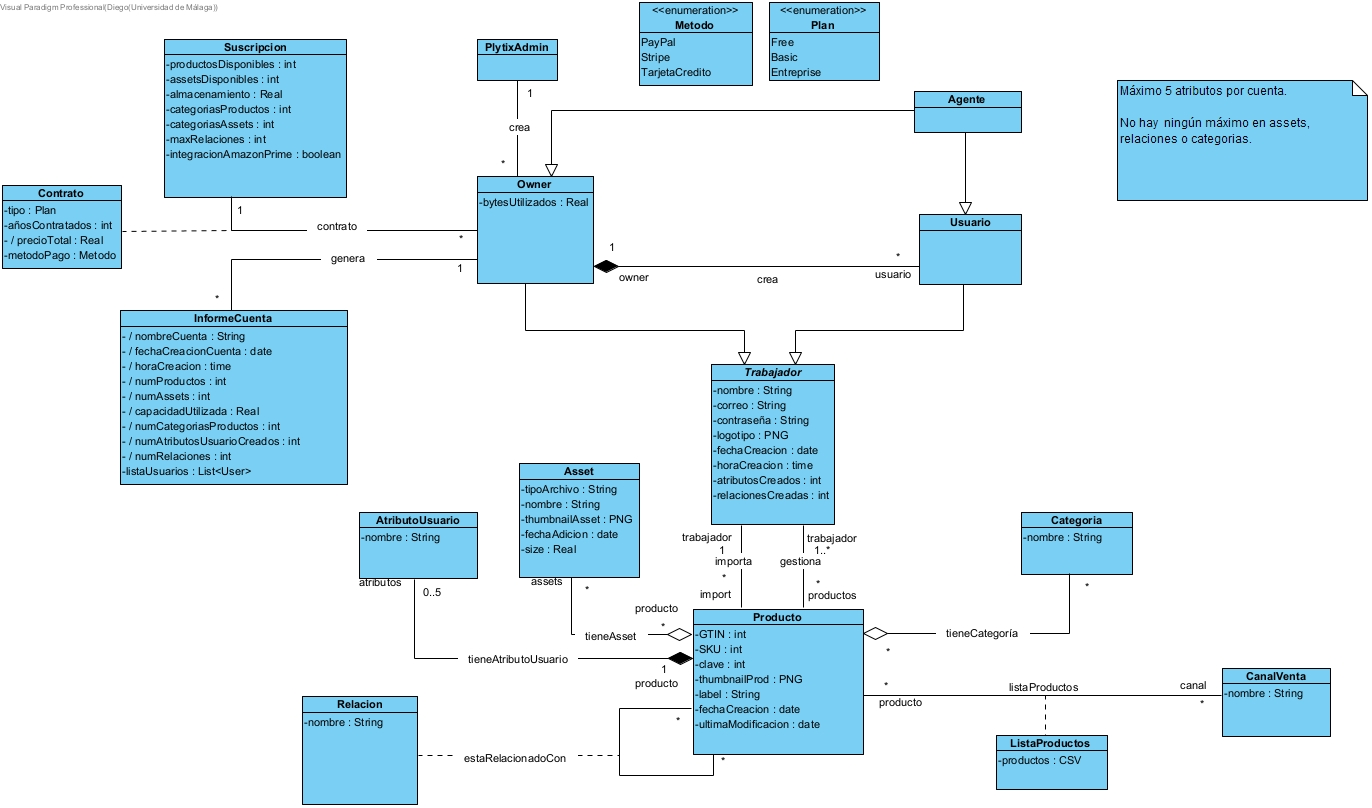
\includegraphics[width=0.8\textwidth]{clases.jpg} % Reduce el ancho al 90% del área de texto
    \caption{Modelo del Dominio}
    \label{fig:mi_imagen}
\end{figure}

\subsection{Trabajador}
    \text{(Clase abstracta)} \textbf{Descripción:}  Clase base para los diferentes tipos de trabajadores, Owner y User. Su propósito es centralizar los atributos comunes a todos los trabajadores.

    \begin{itemize}
        \item {\textbf{Atributos:}}
        \begin{itemize}
            \item \texttt{nombre: String:} Nombre del trabajador.
            \item \texttt{correo: String:} Dirección de correo eléctronico del trabajador.
            \item \texttt{contraseña: String:} Contraseña del trabajador, necesaria para iniciar sesión en el sistema. 
            \item \texttt{logotipo: PNG:} Imagen o logotipo asociado al trabajador, almacenado en formato PNG.
            \item \texttt{fechaCreacion: date:} Fecha en la que se creó el perfil del trabajador en el sistema.
            \item \texttt{horaCreacion: time:} Hora exacta de creación del perfil del trabajador en el sistema. 
            \item \texttt{atributosCreados: int:} Número de atributos creados por el trabajador dentro del sistema. 
            \item \texttt{relacionesCreadas: int:} Número de relaciones que el trabajador ha establecido o creado en el sistema.
        \end{itemize}
    \end{itemize}
    
\subsection{Usuario}
    \text{(Subclase de Trabajador)} \textbf{Descripción:} Representa la cuenta de un trabajador que no es el dueño, pero tiene permisos para gestionar los productos de la empresa.
    \begin{itemize}
        \item {\textbf{Atributos:}} Hereda los atributos de la clase abstracta Trabajador.
    \end{itemize}

\subsection{Owner}
    \text{(Subclase de Trabajador)} \textbf{Descripción:} Representa la cuenta asociada a la tienda con capacidad de crear cuentas User.
    \begin{itemize}
        \item {\textbf{Atributos:}} Hereda los atributos de la clase abstracta Trabajador.
        \begin{itemize}
            \item \texttt{bytesUtilizados: Real:} Es el total de bytes que se está utilizando en todas las cuentas.
        \end{itemize}
    \end{itemize}

\subsection{PlytixAdmin}
    \textbf{Descripción:} Representa a un administrador de Plytix, crea cuentas Owner.

\subsection{Agente}
    \textbf{Descripción:} Representa a un tipo de cuenta que es capaz de simular cuentas de tipo clase Owner o User.

\subsection{Suscripcion}
    \textbf{Descripción:} Representa un plan de suscripción disponible para los usuarios, incluyendo detalles sobre tipo de plan, método de pago, límites de productos y almacenamiento, y opciones de integración.

    \begin{itemize}
        \item {\textbf{Atributos:}}
        \begin{itemize}
            \item \texttt{productosDisponibles: int:} Número de productos que el usuario puede acceder o descargar según su suscripción.
            \item \texttt{assetsDisponibles: int:} Número de elementos gráficos (assets) disponibles para el usuario bajo su plan de suscripción.
            \item \texttt{almacenamiento: int:} Espacio de almacenamiento en GB que el usuario tiene disponible con su suscripción.
            \item \texttt{categoriasProductos: int:} Número de categorías de productos a las que el usuario puede acceder según su tipo de plan.
            \item \texttt{categoriasAssets: int:} Número de categorías de assets accesibles con la suscripción del usuario.
            \item \texttt{maxRelaciones: int:} Cantidad máxima de relaciones que se pueden crear para los productos de la empresa con esta suscripción.
            \item \texttt{integracionAmazonPrime: boolean:} Indica si el plan de suscripción incluye una integración con Amazon Prime.
        \end{itemize}
    \end{itemize}

\subsection{Contrato}
\textbf{Descripción:} Clase de asociación que representa el contrato formal que se crea cuando un usuario Owner paga por una suscripción del sistema.
    \begin{itemize}
        \item {\textbf{Atributos:}}
        \begin{itemize}
            \item \texttt{tipo: Plan:} Tipo de plan de suscripción al que el usuario está suscrito (Free, Basic, Enterprise).
             \item \texttt{añosContratados: int:} Número de años por los cuales el usuario ha contratado la suscripción. Este valor se utiliza para calcular el costo total del contrato.
             \item \texttt{precioTotal: Real (derive):} Precio total del contrato, derivado en base al tipo de plan y los años contratados. Este valor se calcula automáticamente al considerar el costo anual del plan multiplicado por añosContratados.
             \item \texttt{metodoPago: Metodo:} Método de pago utilizado para la suscripción (PayPal, Stripe o TarjetaDeCredito).
        \end{itemize}
    \end{itemize}


\subsection{Metodo}
    \text{(Enumeración)} \textbf{Descripción:} Representa los diferentes métodos de pago disponibles en el sistema (PayPal, Stripe, Tarjeta de Crédito).
    \begin{itemize}
        \item {\textbf{Enumeration Literal:}}
        \begin{itemize}
            \item \texttt{PayPal}
            \item \texttt{Stripe}
            \item \texttt{TarjetaDeCredito}
        \end{itemize}
    \end{itemize}


\subsection{Plan}
    \text{(Enumeración)} \textbf{Descripción:}  Representa los diferentes tipos o categorías de planes disponibles en el sistema (Free, Basic, Enterprise).
    \begin{itemize}
        \item {\textbf{Enumeration Literal:}}
        \begin{itemize}
            \item \texttt{Free}
            \item \texttt{Basic}
            \item \texttt{Enterprise}
        \end{itemize}
    \end{itemize}

\subsection{InformeCuenta}
\textbf{Descripción:} Representa un informe generado para la cuenta Owner en el sistema, proporcionando detalles sobre su creación, uso de recursos, y actividad de usuarios y productos.
    \begin{itemize}
        \item {\textbf{Atributos:}}
        \begin{itemize}
            \item \texttt{nombreCuenta: String (derive):} Nombre de la cuenta para la cual se genera el informe.
            \item \texttt{fechaCreacionCuenta: date (derive):} Fecha en la que se creó la cuenta.
            \item \texttt{horaCreacion: time (derive):} Hora exacta de creación de la cuenta.
            \item \texttt{numProductos: int (derive):} Número total de productos creados por la cuenta.
            \item \texttt{numAssets: int (derive):} Número total de assets asociados a la cuenta.
            \item \texttt{capacidadUtilizada: Real (derive):} Cantidad de almacenamiento utilizado por la cuenta, en unidades de almacenamiento.
            \item \texttt{numCategoriasProductos: int (derive):} Número de categorías creadas en la cuenta.
            \item \texttt{numAtributosUsuariosCreados: int (derive):} Número de atributos creados por los usuarios de la cuenta.
            \item \texttt{numRelaciones: int (derive):} Número de relaciones establecidas en la cuenta.
            \item \texttt{listaUsuarios: List<User>:} Lista de usuarios asociados a la cuenta que han sido previamente creados por el Owner.
        \end{itemize}
    \end{itemize}

\subsection{Producto}
\textbf{Descripción:} Representa un producto que puede ser importado y gestionado por un Trabajador. Incluye identificadores únicos, detalles de creación y fechas de actualización.
    \begin{itemize}
        \item {\textbf{Atributos:}}
        \begin{itemize}
            \item \texttt{GTIN: int:} Código de 14 dígitos que sirve como identificador global del producto (Global Trade Item Number), utilizado para el comercio internacional.
            \item \texttt{SKU: int:} Código de identificación interna que permite rastrear y gestionar el inventario del producto dentro del sistema (Stock Keeping Unit), facilitando su localización y manejo.
            \item \texttt{clave: int:} Valor asignado al producto dentro del sistema, utilizado para referenciar y acceder a la información específica del producto.
            \item \texttt{thumbnailProd: PNG:} Miniatura en formato PNG que representa visualmente el producto.
            \item \texttt{label: String:} Etiqueta que describe o categoriza el producto.
            \item \texttt{fechaCreacion: date:} Fecha en la que se creó el producto en el sistema.
            \item \texttt{ultimaModificacion: date:} Fecha de la última modificación realizada en la información del producto.
        \end{itemize}
    \end{itemize}

\subsection{Relacion}
\textbf{Descripción:} Clase de asociación que representa una relación que crea un usuario entre dos productos.
    \begin{itemize}
        \item {\textbf{Atributos:}}
        \begin{itemize}
            \item \texttt{nombre: String:} Nombre de la relación.
        \end{itemize}
    \end{itemize}

\subsection{AtributoUsuario}
\textbf{Descripción:} Representa un atributo que crea un trabajador y que se atribuye a un producto. Un atributo no puede existir sin el producto al que se le atribuye.
    \begin{itemize}
        \item {\textbf{Atributos:}}
        \begin{itemize}
            \item \texttt{nombre: String:} Nombre del atributo definido por el usuario. No pueden ser más  de 5 por cuenta.
        \end{itemize}
    \end{itemize}

\subsection{Asset}
\textbf{Descripción:} Representa un recurso digital en el sistema que crea un trabajador y que se puede relacionar a varios productos a la vez.
    \begin{itemize}
        \item {\textbf{Atributos:}}
        \begin{itemize}
            \item \texttt{tipoArchivo: String:} Tipo de archivo del asset.
            \item \texttt{nombre: String:} Nombre descriptivo del asset.
            \item \texttt{thumbnailAsset: PNG} Miniatura en formato PNG que representa visualmente al asset.
            \item \texttt{fechaAdicion: date:} Fecha en la que el asset fue añadido al sistema.
            \item \texttt{size: Real:} Tamaño del asset en unidades de almacenamiento.
        \end{itemize}
    \end{itemize}

\subsection{Categoria}
\textbf{Descripción:} Representa una categoría que crea un trabajador y que se puede relacionar a varios productos a la vez.
    \begin{itemize}
        \item {\textbf{Atributos:}}
        \begin{itemize}
            \item \texttt{nombre: String:} Nombre de la categoría.
        \end{itemize}
    \end{itemize}

\subsection{CanalVenta}
\textbf{Descripción:} Representa un canal de venta externo.
    \begin{itemize}
        \item {\textbf{Atributos:}}
        \begin{itemize}
            \item \texttt{nombre: String:} Nombre del canal de venta.
        \end{itemize}
    \end{itemize}

\subsection{ListaProductos}
\textbf{Descripción:} Clase de asociación entre Producto y CanalVenta que representa la lista de productos generada para exportar a un canal de venta en formato CSV.
    \begin{itemize}
        \item {\textbf{Atributos:}}
        \begin{itemize}
            \item \texttt{productos: CSV:} Contenido de la lista de productos en formato CSV.
        \end{itemize}
    \end{itemize}    

\end{document}